\section{Visualizing Tabular Data}
\begin{multicols*}{2}

The Software Carpentry Python course suggests using the \mintinline{python}{matplotlib} library for charts and graphs. This is a decent library for simple charts and graphs, though for anything more sophisticated you might want to look into \mintinline{python}{seaborn}.

\textbf{Important Reminder:} Just like with \texttt{numpy}, you will have to install \texttt{matplotlib} before proceeding:

\vspace{-4mm}
\begin{minted}[xleftmargin=6mm,frame=lines,framesep=2mm,linenos]{bash}
deactivate && source .venv/bin/activate
python3 -m pip install matplotlib
\end{minted}

\subsection{Heatmap with \texttt{imshow}}

Assuming we still have \mintinline{python}{data} set up as the CSV numpy array from the previous section, we can generate a heatmap simply with:

\vspace{-4mm}
\begin{minted}[xleftmargin=6mm,frame=lines,framesep=2mm,linenos]{python}
import matplotlib.pyplot
image = matplotlib.pyplot.imshow(data)
matplotlib.pyplot.savefig('imshow_output.png')
matplotlib.pyplot.show()
\end{minted}

Note that the line 4 only works if you are running Python in a graphical environment: it shows a pop-up with the graphic. \textbf{This is not the case if you are running Python in a Linux shell inside WSL 1.} In that situation, you can remove line 4 and just use the \mintinline{bash}{imshow_output.png} file generated in line 3.

\subsection{Graphing with \texttt{plot}}

The \texttt{matplotlib} library also draws simple line graphs. For example, recalling that each column in this dataset is a day's worth of data, \textbf{``axis 0'' means columns}, we could graph the trend of the daily average inflammation:

\vspace{-4mm}
\begin{minted}[xleftmargin=6mm,frame=lines,framesep=2mm,linenos]{python}
ave_inflammation = numpy.mean(data, axis=0)
ave_plot = matplotlib.pyplot.plot(ave_inflammation)
matplotlib.pyplot.savefig('plot_output.png')
\end{minted}

\subsection{Drawing a \texttt{figure}}
\label{ch3_figure}

\par
You might recall some rules about proper charts and graphs: you should always include a title; you should always label the axes. You may also wish to combine multiple charts and graphs into a single picture. All the above can be achieved using \texttt{figure}.

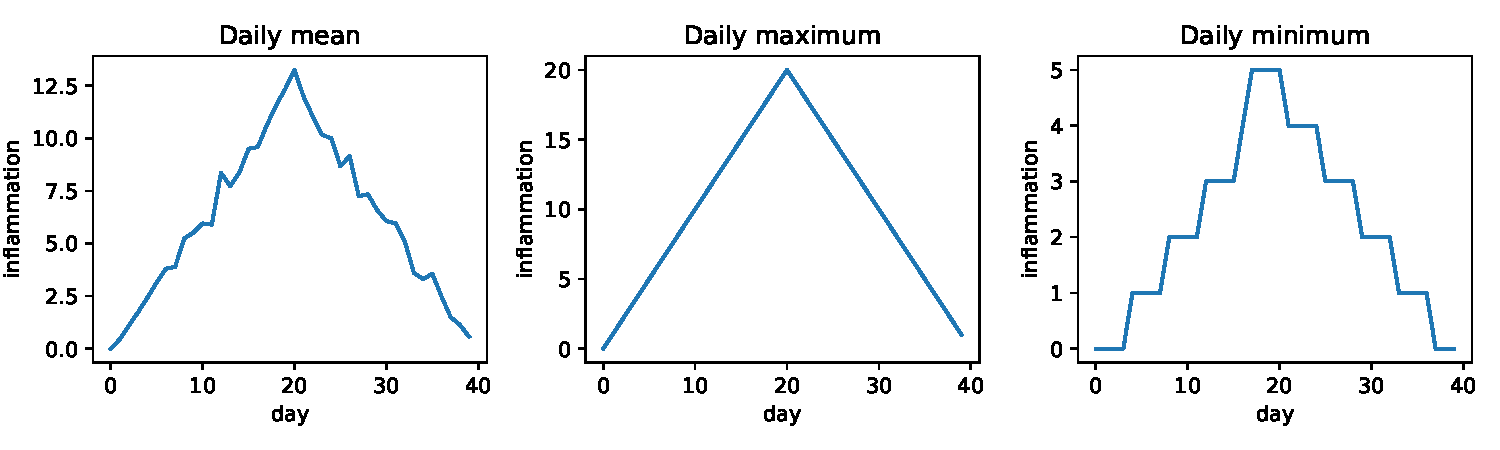
\includegraphics[width=\linewidth]{graphics/inflammation_figure.pdf}

\vspace{-4mm}
\begin{minted}[xleftmargin=6mm,frame=lines,framesep=2mm,linenos,fontsize=\small]{python}
fig = matplotlib.pyplot.figure(figsize=(10.0, 3.0))

axes1 = fig.add_subplot(1, 3, 1); axes1.set_title('Daily mean')
axes1.set_xlabel('day'); axes1.set_ylabel('inflammation')
axes1.plot(numpy.mean(data, axis=0))

axes2 = fig.add_subplot(1, 3, 2); axes2.set_title('Daily maximum')
axes2.set_xlabel('day'); axes2.set_ylabel('inflammation')
axes2.plot(numpy.max(data, axis=0))

axes3 = fig.add_subplot(1, 3, 3); axes3.set_title('Daily minimum')
axes3.set_xlabel('day'); axes3.set_ylabel('inflammation')
axes3.plot(numpy.min(data, axis=0))

fig.tight_layout()
matplotlib.pyplot.savefig('inflammation_figure.pdf')
\end{minted}

Notice that we saved the image as PDF file on line 16. This is exceptionally useful since the resulting PDF file is a vector graphic, not a bitmap. I have actually included this image above - try selecting ``daily maximum'' with your mouse, or try zooming in and seeing how there is no ``pixellation''.

\end{multicols*}